\documentclass[12pt,a4paper]{article}

% --- Настройка языка и шрифтов для LuaLaTeX ---
\usepackage{fontspec}
\defaultfontfeatures{Ligatures=TeX,Scale=MatchLowercase}

\setmainfont{Alice-Regular}[
    Path=font/,
    Extension=.ttf,
    BoldFont = Alice-Regular,
    ItalicFont = Alice-Regular,
    BoldItalicFont = Alice-Regular,
    BoldFeatures = {FakeBold=1.6},
    ItalicFeatures = {FakeSlant=0.2},
    BoldItalicFeatures = {FakeBold=1.6,FakeSlant=0.2}
]

\newfontfamily\cyrillicfont{Alice-Regular}[
    Path=font/,
    Extension=.ttf,
    BoldFont = Alice-Regular,
    ItalicFont = Alice-Regular,
    BoldItalicFont = Alice-Regular,
    BoldFeatures = {FakeBold=1.6},
    ItalicFeatures = {FakeSlant=0.2},
    BoldItalicFeatures = {FakeBold=1.6,FakeSlant=0.2}
]

\usepackage{polyglossia}
\setmainlanguage{russian}
\setsansfont{TeX Gyre Heros}
\setmonofont{TeX Gyre Cursor}

\usepackage{graphicx}        					          % Графика
\usepackage[protrusion=false]{microtype}       	% Микротипографика
\usepackage{amsmath, amsfonts, amssymb, amsthm}	% Математика
\usepackage{braket} 							              % Braket нотация для квантовой механики
\usepackage{unicode-math} 						          % Современный пакет для математики в LuaLaTeX
\usepackage{longtable}       					          % Таблицы с разрывом страниц
\usepackage{tikz}           					          % Рисование
\usepackage[europeanresistors]{circuitikz}		  % Рисование электрических схем в европейском стиле
\usepackage{listings}							              % Для отображения кода
\usepackage{tabularx}       					          % Для таблиц во всю ширину
\usepackage{array}		  						            % Для расширенных возможностей таблиц
\usepackage{float}          					          % Для точного позиционирования фигур
\usepackage{pgfplots}                           % Для построения графиков
\usepackage{caption}                            % Для настройки подписей к рисункам и таблицам
\usepackage{xfp}                                % Для вычислений в LaTeX
\pgfplotsset{compat=1.18}
\usepackage[a4paper,left=20mm,right=20mm,top=20mm,bottom=20mm]{geometry}

\usetikzlibrary{arrows.meta}

% --- Колонтитулы ---
\usepackage{fancyhdr}
\pagestyle{fancy}
\fancyhf{}

\renewcommand{\headrulewidth}{0.4pt}
\renewcommand{\footrulewidth}{0.4pt}
\renewcommand\lstlistingname{Исходный код}

\lstdefinestyle{main}{
	backgroundcolor=\color{gray!8},   
	commentstyle=\color{green!50!black},
	keywordstyle=\color{blue!80!black},
	numberstyle=\small\color{darkgray},
	stringstyle=\rmfamily\color{orange!90!black},
	basicstyle=\ttfamily\small,
	breakatwhitespace=false,         
	breaklines=true,                   
	keepspaces=true,                 
	numbers=left,                    
	numbersep=8pt,                  
	showspaces=false,                
	showstringspaces=false,
	showtabs=false,                  
	tabsize=4
}	

\lstset{style=main}

\newcolumntype{C}{>{\centering\arraybackslash}X}
\renewcommand{\arraystretch}{1.25}

% =========================================================
%         СЛУЖЕБНЫЕ КОМАНДЫ ДЛЯ ВЫЧИСЛЕНИЙ
% =========================================================
\newcommand{\CalcTwo}  [1]{\fpeval{round((#1),2)}}
\newcommand{\CalcThree}[1]{\fpeval{round((#1),3)}}
\newcommand{\CalcFour} [1]{\fpeval{round((#1),4)}}
\newcommand{\CalcFive} [1]{\fpeval{round((#1),5)}}

% ---------------------------------------------------------
% ОБЩИЕ ДАННЫЕ
% ---------------------------------------------------------
\def\VariantN{1}          					         % Номер варианта
\def\StudentName{Андреев Иван Алексеевич}  	 % ФИО студента
\def\TeacherName{NOTHING} % ФИО преподавателя
\def\LabNumber{3}							               % Номер лабораторной работы
\def\Discipline{Атомная физика}				           % Название дисциплины
\def\LabTitle{Изучение термоэлектронной эмиссии и определение работы выхода}	 % Название лабораторной работы

\def\IoneFive       {\fpeval{1 * 10^(-3)}}
\def\IoneTen        {\fpeval{2 * 10^(-3)}}
\def\IoneFifteen    {\fpeval{2 * 10^(-3)}}
\def\IoneTwenty     {\fpeval{2 * 10^(-3)}}
\def\IoneTwentyFive {\fpeval{2 * 10^(-3)}}
\def\IoneThirty     {\fpeval{2 * 10^(-3)}}
\def\IoneThirtyFive {\fpeval{2 * 10^(-3)}}
\def\IoneFortyFive  {\fpeval{3 * 10^(-3)}}
\def\IoneFiftyFive  {\fpeval{3 * 10^(-3)}}
\def\IoneSixtyFive  {\fpeval{3 * 10^(-3)}}
\def\IoneSeventyFive{\fpeval{4 * 10^(-3)}}

\def\ItwoFive       {\fpeval{1 * 10^(-3)}}
\def\ItwoTen        {\fpeval{4 * 10^(-3)}}
\def\ItwoFifteen    {\fpeval{6 * 10^(-3)}}
\def\ItwoTwenty     {\fpeval{7 * 10^(-3)}}
\def\ItwoTwentyFive {\fpeval{7 * 10^(-3)}}
\def\ItwoThirty     {\fpeval{8 * 10^(-3)}}
\def\ItwoThirtyFive {\fpeval{8 * 10^(-3)}}
\def\ItwoFortyFive  {\fpeval{8 * 10^(-3)}}
\def\ItwoFiftyFive  {\fpeval{8 * 10^(-3)}}
\def\ItwoSixtyFive  {\fpeval{8 * 10^(-3)}}
\def\ItwoSeventyFive{\fpeval{8 * 10^(-3)}}

\def\IthreeFive       {\fpeval{2 * 10^(-3)}}
\def\IthreeTen        {\fpeval{4 * 10^(-3)}}
\def\IthreeFifteen    {\fpeval{8 * 10^(-3)}}
\def\IthreeTwenty     {\fpeval{12 * 10^(-3)}}
\def\IthreeTwentyFive {\fpeval{14 * 10^(-3)}}
\def\IthreeThirty     {\fpeval{16 * 10^(-3)}}
\def\IthreeThirtyFive {\fpeval{18 * 10^(-3)}}
\def\IthreeFortyFive  {\fpeval{18 * 10^(-3)}}
\def\IthreeFiftyFive  {\fpeval{19 * 10^(-3)}}
\def\IthreeSixtyFive  {\fpeval{20 * 10^(-3)}}
\def\IthreeSeventyFive{\fpeval{20 * 10^(-3)}}

\def\IsatOne{\IoneSeventyFive}
\def\IsatTwo{\fpeval{6 * 10^(-3)}}
\def\IsatThree{\ItwoSeventyFive}
\def\IsatFour{\fpeval{13 * 10^(-3)}}
\def\IsatFive{\IthreeSeventyFive}

\def\InOne{\fpeval{1.60}}
\def\InTwo{\fpeval{1.65}}
\def\InThree{\fpeval{1.70}}
\def\InFour{\fpeval{1.75}}
\def\InFive{\fpeval{1.80}}

\def\UoneN  {3.3}
\def\UtwoN  {3.5}
\def\UthreeN{3.8}
\def\UfourN {4.0}
\def\UfiveN {4.2}

\def\alphaZero{0.0048}
\def\Rzero{0.25}

\title{
	МИНОБРНАУКИ РОССИИ

	федеральное государственное автономное образовательное учреждение

	высшего образования

	«Национальный исследовательский университет
	«Московский институт электронной техники»
	\vspace{2em}
}
\author{
}
\date{}

\begin{document}

\maketitle
\thispagestyle{fancy} 

\vspace{12em}

\begin{table}[h]
\noindent
\begin{tabular*}{\textwidth}{@{\extracolsep{\fill}} p{0.48\textwidth} p{0.52\textwidth}}
Студент, группа & \StudentName, ЭН-$25$ \\
[0.5em] Руководитель & \TeacherName
\end{tabular*}
\end{table}

\cfoot{Москва 2026}

\pagebreak

\fancyhead[L]{\LabTitle} 
\fancyhead[R]{\Discipline}
\fancyfoot[C]{\thepage}

\begin{center}
	\begin{tabularx}{\textwidth}{|p{1cm}|C|C|C|C|C|C|C|C|C|C|C|}
		\hline
		$U_A$, В & $5$ & $10$ & $15$ & $20$ & $25$ & $30$ & $35$ & $45$ & $55$ & $65$ & $75$ \\
		\hline
	\end{tabularx}
	\begin{tabularx}{\textwidth}{|C p{2cm}|}
		$I_\text{н} = \InOne 0$ A & $U_\text{н} = \UoneN$ В
	\end{tabularx}
	\begin{tabularx}{\textwidth}{|p{1cm}|C|C|C|C|C|C|C|C|C|C|C|}
		\hline
		$I_A$, A & $\fpeval{\IoneFive * 10^3}$ & $\fpeval{\IoneTen * 10^3}$ & $\fpeval{\IoneFifteen * 10^3}$ & $\fpeval{\IoneTwenty * 10^3}$ & $\fpeval{\IoneTwentyFive * 10^3}$ & $\fpeval{\IoneThirty * 10^3}$ & $\fpeval{\IoneThirtyFive * 10^3}$ & $\fpeval{\IoneFortyFive * 10^3}$ & $\fpeval{\IoneFiftyFive * 10^3}$ & $\fpeval{\IoneSixtyFive * 10^3}$ & $\fpeval{\IoneSeventyFive * 10^3}$ \\
		\hline
	\end{tabularx}
	\begin{tabularx}{\textwidth}{|C p{2cm}|}
		$I_\text{н} = \InThree 0$ A & $U_\text{н} = \UthreeN$ В
	\end{tabularx}
	\begin{tabularx}{\textwidth}{|p{1cm}|C|C|C|C|C|C|C|C|C|C|C|}
		\hline
		$I_A$, A & $\fpeval{\ItwoFive * 10^3}$ & $\fpeval{\ItwoTen * 10^3}$ & $\fpeval{\ItwoFifteen * 10^3}$ & $\fpeval{\ItwoTwenty * 10^3}$ & $\fpeval{\ItwoTwentyFive * 10^3}$ & $\fpeval{\ItwoThirty * 10^3}$ & $\fpeval{\ItwoThirtyFive * 10^3}$ & $\fpeval{\ItwoFortyFive * 10^3}$ & $\fpeval{\ItwoFiftyFive * 10^3}$ & $\fpeval{\ItwoSixtyFive * 10^3}$ & $\fpeval{\ItwoSeventyFive * 10^3}$ \\
		\hline
	\end{tabularx}
	\begin{tabularx}{\textwidth}{|C p{2cm}|}
		$I_\text{н} = \InFive 0$ A & $U_\text{н} = \UfiveN$ В
	\end{tabularx}
	\begin{tabularx}{\textwidth}{|p{1cm}|C|C|C|C|C|C|C|C|C|C|C|}
		\hline
		$I_A$, A & $\fpeval{\IthreeFive * 10^3}$ & $\fpeval{\IthreeTen * 10^3}$ & $\fpeval{\IthreeFifteen * 10^3}$ & $\fpeval{\IthreeTwenty * 10^3}$ & $\fpeval{\IthreeTwentyFive * 10^3}$ & $\fpeval{\IthreeThirty * 10^3}$ & $\fpeval{\IthreeThirtyFive * 10^3}$ & $\fpeval{\IthreeFortyFive * 10^3}$ & $\fpeval{\IthreeFiftyFive * 10^3}$ & $\fpeval{\IthreeSixtyFive * 10^3}$ & $\fpeval{\IthreeSeventyFive * 10^3}$ \\
		\hline
	\end{tabularx}
\end{center}

\begin{center}
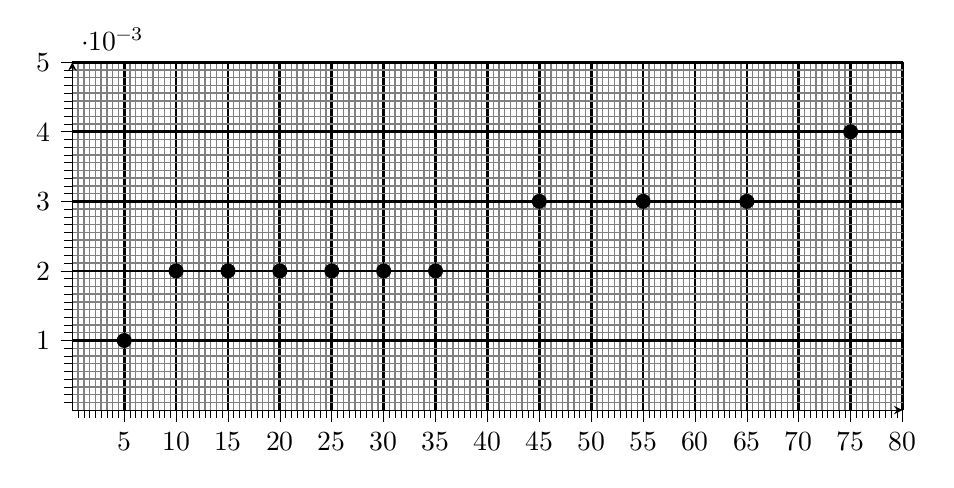
\begin{tikzpicture}
\begin{axis}[
	width=\textwidth,
	height=6cm,
	xmin=0,
	xmax=80,
	ymin=0,
	ymax=5e-3,
	scaled y ticks=base 10:3,
	y tick scale label code/.code={\times10^{-3}},
	axis lines=middle,
	xtick={0,5,...,80},
	ytick={0,0.001,0.002,0.003,0.004,0.005},
	minor x tick num=8,
	minor y tick num=8,
	grid=both,
	major grid style={line width=1pt, draw=black!100},
	minor grid style={line width=0.5pt, draw=black!50},
	xticklabel style={/pgf/number format/fixed,/pgf/number format/precision=1},
	yticklabel style={/pgf/number format/fixed,/pgf/number format/precision=0},
	tick align=outside,
	tick style={black},
]

% Экспериментальные точки
\addplot[
    only marks,
    mark=*,
    mark size=2.5pt
]
coordinates {
    (5, \IoneFive)
	(10, \IoneTen)
	(15, \IoneFifteen)
	(20, \IoneTwenty)
	(25, \IoneTwentyFive)
	(30, \IoneThirty)
	(35, \IoneThirtyFive)
	(45, \IoneFortyFive)
	(55, \IoneFiftyFive)
	(65, \IoneSixtyFive)
	(75, \IoneSeventyFive)
};

\addplot[
    only marks,
    mark=|,
    mark size=5pt
]
coordinates {
    (5 + 0,\IoneFive)
    (10 + 0,\IoneTen)
    (15 + 0,\IoneFifteen)
    (20 + 0,\IoneTwenty)
	(25 + 0,\IoneTwentyFive)
	(30 + 0,\IoneThirty)
	(35 + 0,\IoneThirtyFive)
	(45 + 0,\IoneFortyFive)
	(55 + 0,\IoneFiftyFive)
	(65 + 0,\IoneSixtyFive)
	(75 + 0,\IoneSeventyFive)
	(5 - 0,\IoneFive)
	(10 - 0,\IoneTen)
	(15 - 0,\IoneFifteen)
	(20 - 0,\IoneTwenty)
	(20 - 0,\IoneTwentyFive)
	(25 - 0,\IoneTwentyFive)
	(30 - 0,\IoneThirty)
	(35 - 0,\IoneThirtyFive)
	(45 - 0,\IoneFortyFive)
	(55 - 0,\IoneFiftyFive)
	(65 - 0,\IoneSixtyFive)
	(75 - 0,\IoneSeventyFive)
};

\end{axis}
\end{tikzpicture}
\end{center}

\begin{center}
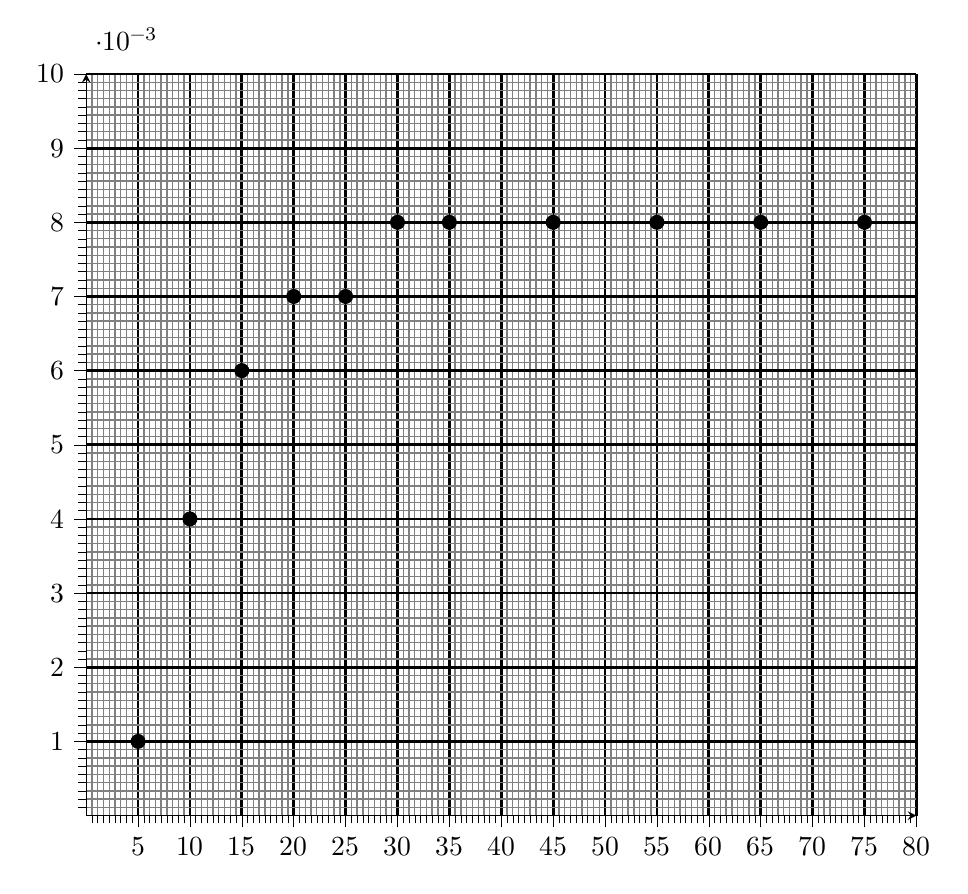
\begin{tikzpicture}
\begin{axis}[
	width=\textwidth,
	height=11cm,
	xmin=0,
	xmax=80,
	ymin=0,
	ymax=10e-3,
	scaled y ticks=base 10:3,
	y tick scale label code/.code={\times10^{-3}},
	axis lines=middle,
	xtick={0,5,...,80},
	ytick={0,0.001,0.002,0.003,0.004,0.005,0.006,0.007,0.008,0.009,0.010},
	minor x tick num=8,
	minor y tick num=8,
	grid=both,
	major grid style={line width=1pt, draw=black!100},
	minor grid style={line width=0.5pt, draw=black!50},
	xticklabel style={/pgf/number format/fixed,/pgf/number format/precision=1},
	yticklabel style={/pgf/number format/fixed,/pgf/number format/precision=0},
	tick align=outside,
	tick style={black},
]

% Экспериментальные точки
\addplot[
    only marks,
    mark=*,
    mark size=2.5pt
]
coordinates {
    (5, \ItwoFive)
	(10, \ItwoTen)
	(15, \ItwoFifteen)
	(20, \ItwoTwenty)
	(25, \ItwoTwentyFive)
	(30, \ItwoThirty)
	(35, \ItwoThirtyFive)
	(45, \ItwoFortyFive)
	(55, \ItwoFiftyFive)
	(65, \ItwoSixtyFive)
	(75, \ItwoSeventyFive)
};

\addplot[
    only marks,
    mark=|,
    mark size=5pt
]
coordinates {
    (5 + 0,\ItwoFive)
    (10 + 0,\ItwoTen)
    (15 + 0,\ItwoFifteen)
    (20 + 0,\ItwoTwenty)
	(25 + 0,\ItwoTwentyFive)
	(30 + 0,\ItwoThirty)
	(35 + 0,\ItwoThirtyFive)
	(45 + 0,\ItwoFortyFive)
	(55 + 0,\ItwoFiftyFive)
	(65 + 0,\ItwoSixtyFive)
	(75 + 0,\ItwoSeventyFive)
	(5 - 0,\ItwoFive)
	(10 - 0,\ItwoTen)
	(15 - 0,\ItwoFifteen)
	(20 - 0,\ItwoTwenty)
	(20 - 0,\ItwoTwentyFive)
	(25 - 0,\ItwoTwentyFive)
	(30 - 0,\ItwoThirty)
	(35 - 0,\ItwoThirtyFive)
	(45 - 0,\ItwoFortyFive)
	(55 - 0,\ItwoFiftyFive)
	(65 - 0,\ItwoSixtyFive)
	(75 - 0,\ItwoSeventyFive)
};

\end{axis}
\end{tikzpicture}
\end{center}

\begin{center}
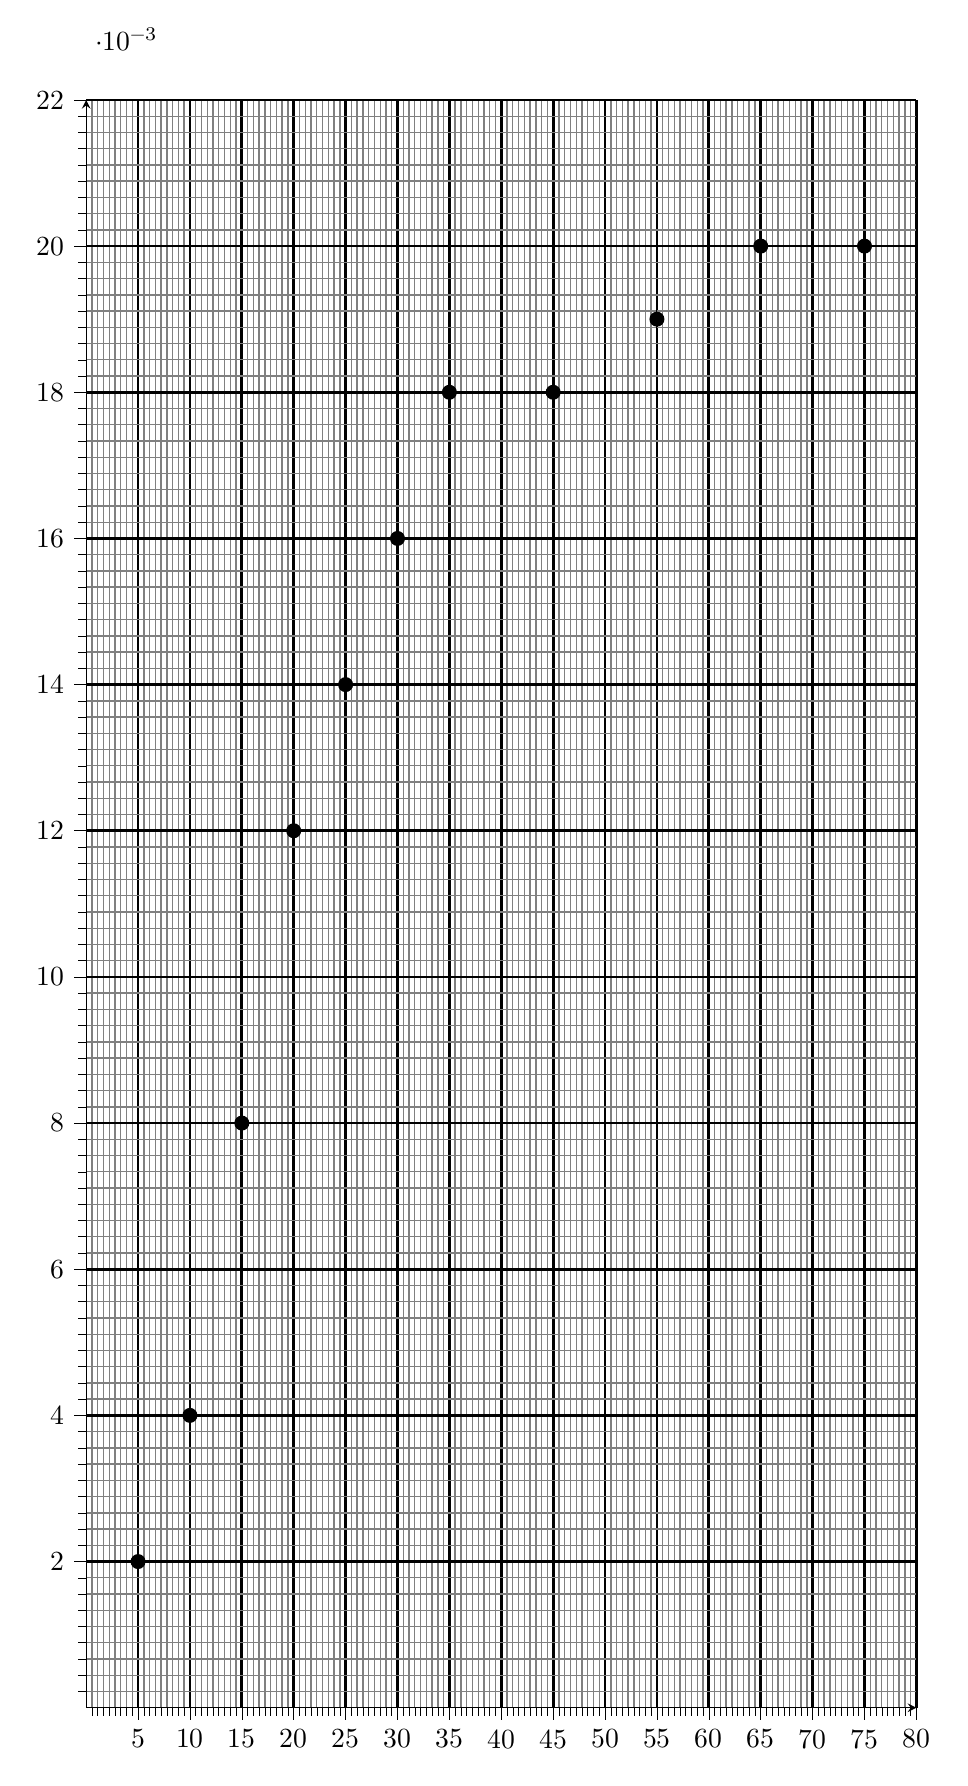
\begin{tikzpicture}
\begin{axis}[
	width=\textwidth,
	height=22cm,
	xmin=0,
	xmax=80,
	ymin=0,
	ymax=22e-3,
	scaled y ticks=base 10:3,
	y tick scale label code/.code={\times10^{-3}},
	axis lines=middle,
	xtick={0,5,...,80},
	ytick={0,2e-3,...,22e-3},
	minor x tick num=8,
	minor y tick num=8,
	grid=both,
	major grid style={line width=1pt, draw=black!100},
	minor grid style={line width=0.5pt, draw=black!50},
	xticklabel style={/pgf/number format/fixed,/pgf/number format/precision=1},
	yticklabel style={/pgf/number format/fixed,/pgf/number format/precision=0},
	tick align=outside,
	tick style={black},
]

% Экспериментальные точки
\addplot[
    only marks,
    mark=*,
    mark size=2.5pt
]
coordinates {
    (5, \IthreeFive)
	(10, \IthreeTen)
	(15, \IthreeFifteen)
	(20, \IthreeTwenty)
	(25, \IthreeTwentyFive)
	(30, \IthreeThirty)
	(35, \IthreeThirtyFive)
	(45, \IthreeFortyFive)
	(55, \IthreeFiftyFive)
	(65, \IthreeSixtyFive)
	(75, \IthreeSeventyFive)
};

\addplot[
    only marks,
    mark=|,
    mark size=5pt
]
coordinates {
    (5 + 0,\IthreeFive)
    (10 + 0,\IthreeTen)
    (15 + 0,\IthreeFifteen)
    (20 + 0,\IthreeTwenty)
	(25 + 0,\IthreeTwentyFive)
	(30 + 0,\IthreeThirty)
	(35 + 0,\IthreeThirtyFive)
	(45 + 0,\IthreeFortyFive)
	(55 + 0,\IthreeFiftyFive)
	(65 + 0,\IthreeSixtyFive)
	(75 + 0,\IthreeSeventyFive)
	(5 - 0,\IthreeFive)
	(10 - 0,\IthreeTen)
	(15 - 0,\IthreeFifteen)
	(20 - 0,\IthreeTwenty)
	(20 - 0,\IthreeTwentyFive)
	(25 - 0,\IthreeTwentyFive)
	(30 - 0,\IthreeThirty)
	(35 - 0,\IthreeThirtyFive)
	(45 - 0,\IthreeFortyFive)
	(55 - 0,\IthreeFiftyFive)
	(65 - 0,\IthreeSixtyFive)
	(75 - 0,\IthreeSeventyFive)
};

\end{axis}
\end{tikzpicture}
\end{center}

\def\RkOne{\fpeval{\UoneN / \InOne}}
\def\RkTwo{\fpeval{\UtwoN / \InTwo}}
\def\RkThree{\fpeval{\UthreeN / \InThree}}
\def\RkFour{\fpeval{\UfourN / \InFour}}
\def\RkFive{\fpeval{\UfiveN / \InFive}}

\def\TOne{\fpeval{(1 / \alphaZero) * ((\RkOne / \Rzero) - 1) + 273}}
\def\TTwo{\fpeval{(1 / \alphaZero) * ((\RkTwo / \Rzero) - 1) + 273}}
\def\TThree{\fpeval{(1 / \alphaZero) * ((\RkThree / \Rzero) - 1) + 273}}
\def\TFour{\fpeval{(1 / \alphaZero) * ((\RkFour / \Rzero) - 1) + 273}}
\def\TFive{\fpeval{(1 / \alphaZero) * ((\RkFive / \Rzero) - 1) + 273}}

\def\TinvertedOne{\fpeval{1 / \TOne}}
\def\TinvertedTwo{\fpeval{1 / \TTwo}}
\def\TinvertedThree{\fpeval{1 / \TThree}}
\def\TinvertedFour{\fpeval{1 / \TFour}}
\def\TinvertedFive{\fpeval{1 / \TFive}}

\def\LnOne{\fpeval{ln(\IsatOne / (\TOne^2))}}
\def\LnTwo{\fpeval{ln(\IsatTwo / (\TTwo^2))}}
\def\LnThree{\fpeval{ln(\IsatThree / (\TThree^2))}}
\def\LnFour{\fpeval{ln(\IsatFour / (\TFour^2))}}
\def\LnFive{\fpeval{ln(\IsatFive / (\TFive^2))}}

% Погрешности исходных величин
\def\DeltaIn{0.05}
\def\DeltaUn{0.1}
\def\DeltaIsat{0.001}

% Погрешности сопротивления катода
\def\DeltaRkOne{\fpeval{\RkOne * sqrt((\DeltaUn / \UoneN)^2 + (\DeltaIn / \InOne)^2)}}
\def\DeltaRkTwo{\fpeval{\RkTwo * sqrt((\DeltaUn / \UtwoN)^2 + (\DeltaIn / \InTwo)^2)}}
\def\DeltaRkThree{\fpeval{\RkThree * sqrt((\DeltaUn / \UthreeN)^2 + (\DeltaIn / \InThree)^2)}}
\def\DeltaRkFour{\fpeval{\RkFour * sqrt((\DeltaUn / \UfourN)^2 + (\DeltaIn / \InFour)^2)}}
\def\DeltaRkFive{\fpeval{\RkFive * sqrt((\DeltaUn / \UfiveN)^2 + (\DeltaIn / \InFive)^2)}}

% Погрешности температуры
\def\DeltaTOne{\fpeval{\DeltaRkOne / (\alphaZero * \Rzero)}}
\def\DeltaTTwo{\fpeval{\DeltaRkTwo / (\alphaZero * \Rzero)}}
\def\DeltaTThree{\fpeval{\DeltaRkThree / (\alphaZero * \Rzero)}}
\def\DeltaTFour{\fpeval{\DeltaRkFour / (\alphaZero * \Rzero)}}
\def\DeltaTFive{\fpeval{\DeltaRkFive / (\alphaZero * \Rzero)}}

% Погрешности обратной температуры
\def\DeltaTinvertedOne{\fpeval{\DeltaTOne / (\TOne^2)}}
\def\DeltaTinvertedTwo{\fpeval{\DeltaTTwo / (\TTwo^2)}}
\def\DeltaTinvertedThree{\fpeval{\DeltaTThree / (\TThree^2)}}
\def\DeltaTinvertedFour{\fpeval{\DeltaTFour / (\TFour^2)}}
\def\DeltaTinvertedFive{\fpeval{\DeltaTFive / (\TFive^2)}}

% Погрешности логарифма
\def\DeltaLnOne{\fpeval{sqrt((\DeltaIsat / \IsatOne)^2 + (2 * \DeltaTOne / \TOne)^2)}}
\def\DeltaLnTwo{\fpeval{sqrt((\DeltaIsat / \IsatTwo)^2 + (2 * \DeltaTTwo / \TTwo)^2)}}
\def\DeltaLnThree{\fpeval{sqrt((\DeltaIsat / \IsatThree)^2 + (2 * \DeltaTThree / \TThree)^2)}}
\def\DeltaLnFour{\fpeval{sqrt((\DeltaIsat / \IsatFour)^2 + (2 * \DeltaTFour / \TFour)^2)}}
\def\DeltaLnFive{\fpeval{sqrt((\DeltaIsat / \IsatFive)^2 + (2 * \DeltaTFive / \TFive)^2)}}

\def\xMaxOne{\fpeval{\TinvertedFive - \DeltaTinvertedFive}}
\def\yMaxOne{\fpeval{\LnFive - \DeltaLnFive}}
\def\xMaxTwo{\fpeval{\TinvertedOne + \DeltaTinvertedOne}}
\def\yMaxTwo{\fpeval{\LnOne + \DeltaLnOne}}

\def\xMinOne{\fpeval{\TinvertedFive + \DeltaTinvertedFive}}
\def\yMinOne{\fpeval{\LnFive + \DeltaLnFive}}
\def\xMinTwo{\fpeval{\TinvertedOne - \DeltaTinvertedOne}}
\def\yMinTwo{\fpeval{\LnOne - \DeltaLnOne}}

\def\GammaMax{\fpeval{(\yMaxTwo - \yMaxOne) / (\xMaxTwo - \xMaxOne)}}
\def\GammaMin{\fpeval{(\yMinTwo - \yMinOne) / (\xMinTwo - \xMinOne)}}

\def\GammaMean{\fpeval{(\GammaMax + \GammaMin) / 2}}
\def\DeltaGamma{\fpeval{abs(\GammaMax - \GammaMin) / 2}}

\def\WorkFunction{\fpeval{-\GammaMean * ((1.38e-23) / (1.6e-19))}}
\def\DeltaWorkFunction{\fpeval{\DeltaGamma * ((1.38e-23) / (1.6e-19))}}

\begin{tabularx}{\textwidth}{|C|C|C|C|C|p{2cm}|p{2.5cm}|p{2cm}|}
	\hline
	$I_\text{н}$, А & $U_\text{н}$, В & $I_\text{нас}$, А & $R_\text{к}$, Ом & $T$, К & 
	$\Delta\left(\frac{1}{T}\right)$, К$^{-1}$ & \centering $\ln{\frac{I_\text{нас}}{T^2}}$ 
	& $\Delta\left(\ln{\frac{I_\text{нас}}{T^2}}\right)$ \\
	\hline
	$\InOne 0$ & $\UoneN$ & $\fpeval{\IsatOne * 1000}$ & $\CalcFour{\RkOne}$ & $\CalcTwo{\TOne}$ & $\CalcTwo{\DeltaTinvertedOne * 10^5} \cdot 10^{-5}$ & $\CalcFour{\LnOne}$ & $\CalcTwo{\DeltaLnOne}$ \\ 
	\hline
	$\InTwo$ & $\UtwoN$ & $\fpeval{\IsatTwo * 1000}$ & $\CalcFour{\RkTwo}$ & $\CalcTwo{\TTwo}$ & $\CalcTwo{\DeltaTinvertedTwo * 10^5} \cdot 10^{-5}$ & $\CalcFour{\LnTwo}$ & $\CalcTwo{\DeltaLnTwo}$ \\
	\hline
	$\InThree 0$ & $\UthreeN$ & $\fpeval{\IsatThree * 1000}$ & $\CalcFour{\RkThree}$ & $\CalcTwo{\TThree}$ & $\CalcTwo{\DeltaTinvertedThree * 10^5} \cdot 10^{-5}$ & $\CalcFour{\LnThree}$ & $\CalcTwo{\DeltaLnThree}$ \\
	\hline
	$\InFour$ & $\UfourN$ & $\fpeval{\IsatFour * 1000}$ & $\CalcFour{\RkFour}$ & $\CalcTwo{\TFour}$ & $\CalcTwo{\DeltaTinvertedFour * 10^5} \cdot 10^{-5}$ & $\CalcFour{\LnFour}$ & $\CalcTwo{\DeltaLnFour}$ \\
	\hline
	$\InFive 0$ & $\UfiveN$ & $\fpeval{\IsatFive * 1000}$ & $\CalcFour{\RkFive}$ & $\CalcTwo{\TFive}$ & $\CalcTwo{\DeltaTinvertedFive * 10^5} \cdot 10^{-5}$ & $\CalcFour{\LnFive}$ & $\CalcTwo{\DeltaLnFive}$ \\
	\hline
\end{tabularx}

\vspace{1em}

\begin{equation*}
	\begin{aligned}
		R_\text{к} = \frac{U_\text{н}}{I_\text{н}} \quad & R_{\text{к}1} = \frac{\UoneN}{\InOne} = \CalcFive{\UoneN / \InOne} \\
												   		 & R_{\text{к}2} = \frac{\UtwoN}{\InTwo} = \CalcFive{\UtwoN / \InTwo} \\
												   		 & R_{\text{к}3} = \frac{\UthreeN}{\InThree} = \CalcFive{\UthreeN / \InThree} \\
												   		 & R_{\text{к}4} = \frac{\UfourN}{\InFour} = \CalcFive{\UfourN / \InFour} \\
												   		 & R_{\text{к}5} = \frac{\UfiveN}{\InFive} = \CalcFive{\UfiveN / \InFive} \\
	\end{aligned}
\end{equation*}

\begin{equation*}
	\begin{aligned}
		T = \frac{1}{\alpha}\left(\frac{R_\text{к}}{R_0} - 1\right) + 273 \quad & T_1 = \frac{1}{\alphaZero}\left(\frac{\CalcFive{\RkOne}}{\Rzero} - 1\right) + 273 = \CalcFive{(1 / \alphaZero) * ((\RkOne / \Rzero) - 1) + 273} \\
												    & T_2 = \frac{1}{\alphaZero}\left(\frac{\CalcFive{\RkTwo}}{\Rzero} - 1\right) + 273 = \CalcFive{(1 / \alphaZero) * ((\RkTwo / \Rzero) - 1) + 273} \\
												    & T_3 = \frac{1}{\alphaZero}\left(\frac{\CalcFive{\RkThree}}{\Rzero} - 1\right) + 273 = \CalcFive{(1 / \alphaZero) * ((\RkThree / \Rzero) - 1) + 273} \\
												    & T_4 = \frac{1}{\alphaZero}\left(\frac{\CalcFive{\RkFour}}{\Rzero} - 1\right) + 273 = \CalcFive{(1 / \alphaZero) * ((\RkFour / \Rzero) - 1) + 273} \\
												    & T_5 = \frac{1}{\alphaZero}\left(\frac{\CalcFive{\RkFive}}{\Rzero} - 1\right) + 273 = \CalcFive{(1 / \alphaZero) * ((\RkFive / \Rzero) - 1) + 273}
	\end{aligned}
\end{equation*}

\begin{equation*}
	\begin{aligned}
		\frac{1}{T} \quad & \frac{1}{\CalcTwo{\TOne}} = \CalcFive{1 / \TOne} \\
						 & \frac{1}{\CalcTwo{\TTwo}} = \CalcFive{1 / \TTwo} \\
						 & \frac{1}{\CalcTwo{\TThree}} = \CalcFive{1 / \TThree} \\
						 & \frac{1}{\CalcTwo{\TFour}} = \CalcFive{1 / \TFour} \\
						 & \frac{1}{\CalcTwo{\TFive}} = \CalcFive{1 / \TFive}
	\end{aligned}
\end{equation*}

\begin{equation*}
	\begin{aligned}
		\ln{\frac{I_\text{нас}}{T^2}} \quad & \ln{\frac{\IsatOne}{\CalcTwo{\TOne}^2}} = \CalcFive{ln(\IsatOne / (\TOne^2))} \\
										   & \ln{\frac{\IsatTwo}{\CalcTwo{\TTwo}^2}} = \CalcFive{ln(\IsatTwo / (\TTwo^2))} \\
										   & \ln{\frac{\IsatThree}{\CalcTwo{\TThree}^2}} = \CalcFive{ln(\IsatThree / (\TThree^2))} \\
										   & \ln{\frac{\IsatFour}{\CalcTwo{\TFour}^2}} = \CalcFive{ln(\IsatFour / (\TFour^2))} \\
										   & \ln{\frac{\IsatFive}{\CalcTwo{\TFive}^2}} = \CalcFive{ln(\IsatFive / (\TFive^2))}
	\end{aligned}
\end{equation*}

\begin{equation*}
	\begin{aligned}
		\Delta R_\text{к} = R_\text{к}\sqrt{\left(\frac{\Delta U_\text{н}}{U_\text{н}}\right)^2 + \left(\frac{\Delta I_\text{н}}{I_\text{н}}\right)^2}
		\quad & \Delta R_{\text{к}1} = \CalcFive{\RkOne}\sqrt{\left(\frac{\DeltaUn}{\UoneN}\right)^2 + \left(\frac{\DeltaIn}{\InOne}\right)^2} = \CalcFive{\DeltaRkOne} \\
		      & \Delta R_{\text{к}2} = \CalcFive{\RkTwo}\sqrt{\left(\frac{\DeltaUn}{\UtwoN}\right)^2 + \left(\frac{\DeltaIn}{\InTwo}\right)^2} = \CalcFive{\DeltaRkTwo} \\
		      & \Delta R_{\text{к}3} = \CalcFive{\RkThree}\sqrt{\left(\frac{\DeltaUn}{\UthreeN}\right)^2 + \left(\frac{\DeltaIn}{\InThree}\right)^2} = \CalcFive{\DeltaRkThree} \\
		      & \Delta R_{\text{к}4} = \CalcFive{\RkFour}\sqrt{\left(\frac{\DeltaUn}{\UfourN}\right)^2 + \left(\frac{\DeltaIn}{\InFour}\right)^2} = \CalcFive{\DeltaRkFour} \\
		      & \Delta R_{\text{к}5} = \CalcFive{\RkFive}\sqrt{\left(\frac{\DeltaUn}{\UfiveN}\right)^2 + \left(\frac{\DeltaIn}{\InFive}\right)^2} = \CalcFive{\DeltaRkFive}
	\end{aligned}
\end{equation*}

\begin{equation*}
	\begin{aligned}
		\Delta T = \frac{\Delta R_\text{к}}{\alpha R_0}
		\quad & \Delta T_1 = \frac{\CalcFive{\DeltaRkOne}}{\alphaZero \cdot \Rzero} = \CalcFive{\DeltaTOne} \\
		      & \Delta T_2 = \frac{\CalcFive{\DeltaRkTwo}}{\alphaZero \cdot \Rzero} = \CalcFive{\DeltaTTwo} \\
		      & \Delta T_3 = \frac{\CalcFive{\DeltaRkThree}}{\alphaZero \cdot \Rzero} = \CalcFive{\DeltaTThree} \\
		      & \Delta T_4 = \frac{\CalcFive{\DeltaRkFour}}{\alphaZero \cdot \Rzero} = \CalcFive{\DeltaTFour} \\
		      & \Delta T_5 = \frac{\CalcFive{\DeltaRkFive}}{\alphaZero \cdot \Rzero} = \CalcFive{\DeltaTFive}
	\end{aligned}
\end{equation*}

\begin{equation*}
	\begin{aligned}
		\Delta\left(\frac{1}{T}\right) = \frac{\Delta T}{T^2}
		\quad & \Delta\left(\frac{1}{T_1}\right) = \frac{\CalcFive{\DeltaTOne}}{\CalcTwo{\TOne}^2} = \CalcFive{\DeltaTinvertedOne} \\
		      & \Delta\left(\frac{1}{T_2}\right) = \frac{\CalcFive{\DeltaTTwo}}{\CalcTwo{\TTwo}^2} = \CalcFive{\DeltaTinvertedTwo} \\
		      & \Delta\left(\frac{1}{T_3}\right) = \frac{\CalcFive{\DeltaTThree}}{\CalcTwo{\TThree}^2} = \CalcFive{\DeltaTinvertedThree} \\
		      & \Delta\left(\frac{1}{T_4}\right) = \frac{\CalcFive{\DeltaTFour}}{\CalcTwo{\TFour}^2} = \CalcFive{\DeltaTinvertedFour} \\
		      & \Delta\left(\frac{1}{T_5}\right) = \frac{\CalcFive{\DeltaTFive}}{\CalcTwo{\TFive}^2} = \CalcFive{\DeltaTinvertedFive}
	\end{aligned}
\end{equation*}

\begin{equation*}
	\begin{aligned}
		\Delta\left(\ln{\frac{I_\text{нас}}{T^2}}\right) =
		\sqrt{\left(\frac{\Delta I_\text{нас}}{I_\text{нас}}\right)^2 + \left(2\frac{\Delta T}{T}\right)^2}
		\quad & \Delta\left(\ln{\frac{I_{\text{нас}1}}{T_1^2}}\right) = \sqrt{\left(\frac{\DeltaIsat}{\IsatOne}\right)^2 + \left(2\frac{\CalcFive{\DeltaTOne}}{\CalcTwo{\TOne}}\right)^2} = \CalcFive{\DeltaLnOne} \\
		      & \Delta\left(\ln{\frac{I_{\text{нас}2}}{T_2^2}}\right) = \sqrt{\left(\frac{\DeltaIsat}{\IsatTwo}\right)^2 + \left(2\frac{\CalcFive{\DeltaTTwo}}{\CalcTwo{\TTwo}}\right)^2} = \CalcFive{\DeltaLnTwo} \\
		      & \Delta\left(\ln{\frac{I_{\text{нас}3}}{T_3^2}}\right) = \sqrt{\left(\frac{\DeltaIsat}{\IsatThree}\right)^2 + \left(2\frac{\CalcFive{\DeltaTThree}}{\CalcTwo{\TThree}}\right)^2} = \CalcFive{\DeltaLnThree} \\
		      & \Delta\left(\ln{\frac{I_{\text{нас}4}}{T_4^2}}\right) = \sqrt{\left(\frac{\DeltaIsat}{\IsatFour}\right)^2 + \left(2\frac{\CalcFive{\DeltaTFour}}{\CalcTwo{\TFour}}\right)^2} = \CalcFive{\DeltaLnFour} \\
		      & \Delta\left(\ln{\frac{I_{\text{нас}5}}{T_5^2}}\right) = \sqrt{\left(\frac{\DeltaIsat}{\IsatFive}\right)^2 + \left(2\frac{\CalcFive{\DeltaTFive}}{\CalcTwo{\TFive}}\right)^2} = \CalcFive{\DeltaLnFive}
	\end{aligned}
\end{equation*}

\begin{center}
\begin{tikzpicture}
\begin{axis}[
    width=\textwidth,
    height=\textwidth,
    xmin=4.7e-4,
    xmax=5.9e-4,
    ymin=-20.8,
    ymax=-19.0,
    axis lines=left,
    enlargelimits=false,
    xlabel={$1/T,\ \mathrm{K^{-1}}$},
    ylabel={$\ln\!\left(\dfrac{I_{\mathrm{нас}}}{T^2}\right)$},
    xtick={4.6e-4,4.8e-4,5.0e-4,5.2e-4,5.4e-4,5.6e-4,5.8e-4, 6.0e-4},
    ytick={-20.8 , -20.6, -20.4, -20.2, -20.0, -19.8, -19.6, -19.4, -19.2, -19.0},
    minor x tick num=8,
    minor y tick num=8,
    grid=both,
    major grid style={draw=black, line width=0.5pt},
    minor grid style={draw=gray!60, line width=0.25pt},
    tick align=outside,
    tick style={black, line width=0.4pt},
    major tick length=3pt,
    minor tick length=1.5pt,
    scaled x ticks=false,
    xticklabels={$4.6$, $4.8$, $5.0$, $5.2$, $5.4$, $5.6$, $5.8$, $6.0$},
    yticklabel style={
        /pgf/number format/fixed,
        /pgf/number format/precision=1
    },
    clip=false
]

% Экспериментальные точки
\addplot[
    only marks,
    mark=*,
    mark size=2.2pt
]
coordinates {
    (\TinvertedOne,   \LnOne)
    (\TinvertedTwo,   \LnTwo)
    (\TinvertedThree, \LnThree)
    (\TinvertedFour,  \LnFour)
    (\TinvertedFive,  \LnFive)
};

\addplot[
	only marks,
	mark=|,
	mark size=5pt
]
coordinates {
    (\TinvertedOne + \DeltaTinvertedOne, \LnOne)
	(\TinvertedTwo + \DeltaTinvertedTwo, \LnTwo)
	(\TinvertedThree + \DeltaTinvertedThree, \LnThree)
	(\TinvertedFour + \DeltaTinvertedFour, \LnFour)
	(\TinvertedFive + \DeltaTinvertedFive, \LnFive)
	(\TinvertedOne - \DeltaTinvertedOne, \LnOne)
	(\TinvertedTwo - \DeltaTinvertedTwo, \LnTwo)
	(\TinvertedThree - \DeltaTinvertedThree, \LnThree)
	(\TinvertedFour - \DeltaTinvertedFour, \LnFour)
	(\TinvertedFive - \DeltaTinvertedFive, \LnFive)
};

\addplot[
	only marks,
	mark=-,
	mark size=5pt
]
coordinates {
	(\TinvertedOne, \LnOne + \DeltaLnOne)
	(\TinvertedTwo, \LnTwo + \DeltaLnTwo)
	(\TinvertedThree, \LnThree + \DeltaLnThree)
	(\TinvertedFour, \LnFour + \DeltaLnFour)
	(\TinvertedFive, \LnFive + \DeltaLnFive)
	(\TinvertedOne, \LnOne - \DeltaLnOne)
	(\TinvertedTwo, \LnTwo - \DeltaLnTwo)
	(\TinvertedThree, \LnThree - \DeltaLnThree)
	(\TinvertedFour, \LnFour - \DeltaLnFour)
	(\TinvertedFive, \LnFive - \DeltaLnFive)
};

\node[anchor=north east] at (rel axis cs:1,0) {$\cdot 10^{-4}$};

\end{axis}
\end{tikzpicture}
\end{center}


\begin{equation*}
	\begin{aligned}
		\gamma_{\max} = \frac{\Delta y}{\Delta x}
		\quad & \gamma_{\max} = \frac{\yMaxTwo - \yMaxOne}{\xMaxTwo - \xMaxOne} = \CalcFive{(\yMaxTwo - \yMaxOne) / (\xMaxTwo - \xMaxOne)}
	\end{aligned}
\end{equation*}

\begin{equation*}
	\begin{aligned}
		\gamma_{\min} = \frac{\Delta y}{\Delta x}
		\quad & \gamma_{\min} = \frac{\yMinTwo - \yMinOne}{\xMinTwo - \xMinOne} = \CalcFive{(\yMinTwo - \yMinOne) / (\xMinTwo - \xMinOne)}
	\end{aligned}
\end{equation*}

\begin{equation*}
	\begin{aligned}
		\gamma_\text{ср} = \frac{\gamma_{\max} + \gamma_{\min}}{2}
		\quad & \gamma_\text{ср} = \frac{\CalcFive{\GammaMax} + \CalcFive{\GammaMin}}{2} = \CalcFive{(\GammaMax + \GammaMin) / 2}
	\end{aligned}
\end{equation*}

\begin{equation*}
	\begin{aligned}
		\Delta \gamma = \frac{|\gamma_{\max} - \gamma_{\min}|}{2}
		\quad & \Delta \gamma = \frac{|\CalcFive{\GammaMax} - \CalcFive{\GammaMin}|}{2} = \CalcFive{abs(\GammaMax - \GammaMin) / 2}
	\end{aligned}
\end{equation*}

\begin{equation*}
	\begin{aligned}
		\gamma = \gamma_\text{ср} \pm \Delta\gamma
		\quad & \gamma = \CalcFive{\GammaMean} \pm \CalcFive{\DeltaGamma}
	\end{aligned}
\end{equation*}

\begin{equation*}
	\begin{aligned}
		\gamma = -\frac{e\varphi}{k} \quad & A = e\varphi = -\gamma k \\
										   & A = -\gamma\frac{k}{e} = -\gamma \cdot \CalcFive{(1.38e-23) / (1.6e-19)}
	\end{aligned}
\end{equation*}

\begin{equation*}
	\begin{aligned}
		A = -\gamma\frac{k}{e} \quad & A = -\CalcFive{\GammaMean}\cdot\CalcFive{(1.38e-23) / (1.6e-19)} = \CalcFive{\WorkFunction}
	\end{aligned}
\end{equation*}

\begin{equation*}
	\begin{aligned}
		\Delta A = \Delta\gamma\frac{k}{e} \quad & \Delta A = \CalcFive{\DeltaGamma}\cdot\CalcFive{(1.38e-23) / (1.6e-19)} = \CalcFive{\DeltaWorkFunction}
	\end{aligned}
\end{equation*}



\end{document}